\chapter{Manuscript 1}\label{chap:manuscript_1}

% Example manuscript-style chapter demonstrating advanced LaTeX features

\section{Introduction}

Maecenas pulvinar, enim aliquam porttitor tempus, dolor nibh accumsan libero, id scelerisque ligula nibh vitae metus. Vivamus fringilla, tellus nec sodales faucibus, ex neque mollis lorem, vel aliquet elit justo et quam. Cras non ultrices eros. Nulla scelerisque suscipit accumsan. Duis neque mi, suscipit et felis quis, finibus tincidunt ex. Etiam non enim ut nulla vehicula vestibulum. Duis ultrices odio a commodo interdum. Fusce lacinia sodales laoreet.

Nulla sit amet vulputate diam. Etiam quis finibus turpis. Vestibulum ac auctor elit, nec faucibus massa. Morbi ullamcorper felis nisi, et elementum nibh porta a. Duis vestibulum orci ex, eget porttitor felis malesuada sed. Phasellus eros arcu, elementum at consequat sed, placerat et velit. Vivamus nisi tellus, placerat sed velit id, pellentesque mattis ex.

\section{Methods}

\subsection*{Participants}

Participants were greater than or equal to, which can also be written as $\geq 18$.

\subsection*{Behavioral Measures}

Integer purus est, hendrerit eget mollis at, maximus in elit. Phasellus eu lacinia eros. In ac ultricies nunc. Aenean malesuada commodo lacus id consectetur. Fusce facilisis hendrerit sem. Nunc sed faucibus tortor. Nullam tincidunt, felis sed mollis hendrerit, massa elit egestas lorem, quis dapibus leo diam quis nibh. Donec neque orci, molestie non velit ut, pulvinar elementum leo. Sed neque quam, ultricies vitae tortor a, tincidunt lacinia libero. Morbi vitae condimentum mauris. Vivamus venenatis erat ullamcorper, fermentum est vel, laoreet magna. Aliquam elementum lorem

\subsection*{Example Figure}

As shown in \textbf{\autoref{fig:example_main}}, figures are included using the standard \texttt{figure} environment.

\begin{figure}[htbp]
\centering
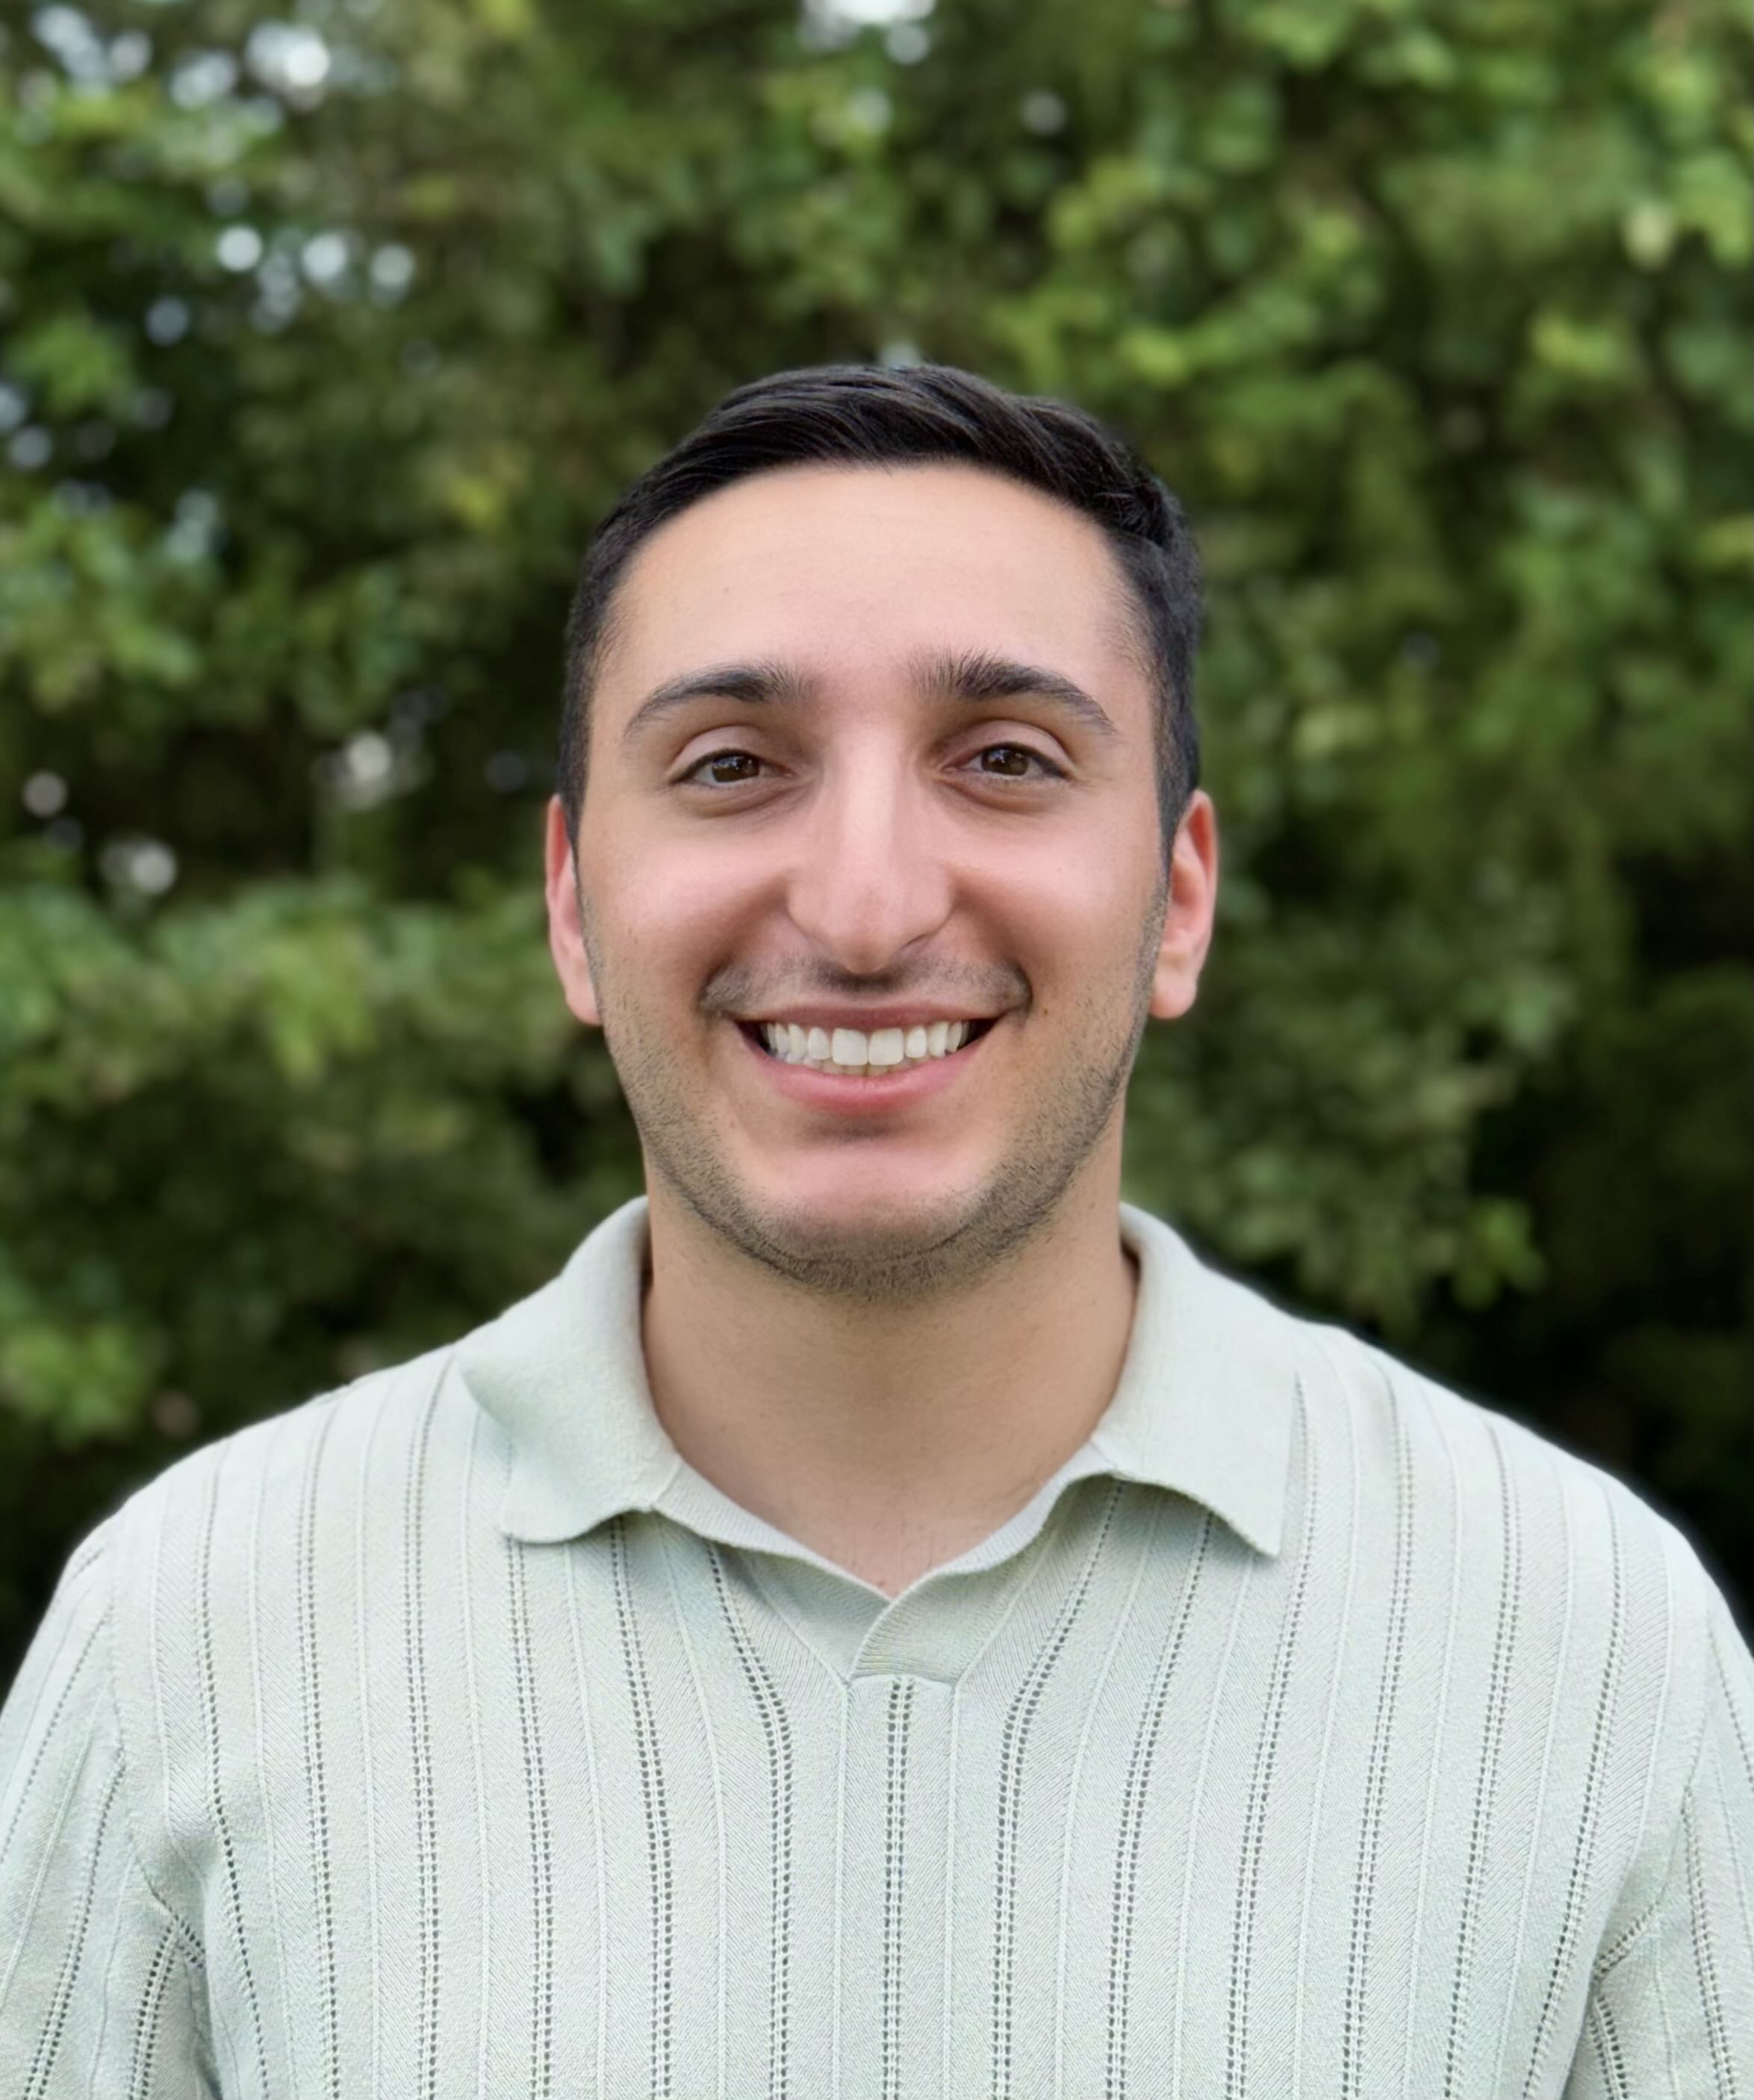
\includegraphics[width=0.3\linewidth]{figures/headshot.png}
\caption[Example figure. Again here is the short caption]{\textbf{Example figure. Again here is the short caption} This demonstrates how to include and reference a figure in a manuscript chapter.}
\label{fig:example_main}
\end{figure}

\subsection*{Example Math}

Inline statistical reporting: $p < 0.05$

Display math:

\[
F_{(1,22)} = 7.12, \quad p < 0.05
\]

\section{Results}

Nulla ut elit lorem. Aenean lorem metus, venenatis sed vehicula eu, rhoncus eu dui. Nam cursus bibendum hendrerit. Phasellus elementum consequat felis ac ornare. Ut eget neque in orci cursus ullamcorper eget vitae urna. Mauris risus mi, tincidunt vitae neque id, auctor dignissim turpis. Integer iaculis blandit lectus pulvinar ullamcorper. Morbi at nulla ac mauris tristique tincidunt eu vitae ante.

 (\textbf{\autoref{fig:example_main}}).

Suspendisse vel tincidunt nunc. Aenean feugiat consectetur augue et sagittis. Vivamus elementum, magna a mollis fringilla, lorem elit posuere (see \textbf{\suppautoref{supfig:example_supp}}).

\section{Discussion}

Suspendisse congue elementum est, non lobortis massa rhoncus a. Nulla facilisi. In in faucibus nisi. Proin metus magna, tristique quis consequat vestibulum, sollicitudin quis diam. Nulla in dapibus mi, vel vulputate diam. In tellus dui, mattis facilisis nulla sed, pulvinar gravida mi. Nullam placerat felis eget diam tincidunt, in vestibulum lectus venenatis. Etiam a viverra massa. Quisque sagittis pulvinar iaculis. Aliquam erat volutpat. Aliquam non condimentum tellus. Nunc vel tortor at tellus cursus ultricies. Donec ut convallis metus.

Vestibulum egestas pellentesque tortor vitae interdum. Vivamus sed nulla ornare, ultricies odio id, aliquam massa. Sed auctor mollis lacus eu cursus. Praesent congue nibh libero, porta finibus lacus eleifend et. In in lectus nec odio sodales accumsan in eget tortor. Suspendisse cursus ligula et diam bibendum, et bibendum enim lacinia. Quisque lobortis augue non congue tincidunt. Duis ut neque a magna fringilla tempus ut non felis. Vivamus auctor leo nec nulla porta malesuada. Maecenas id interdum tortor.

\section{Conclusion}

Nam efficitur euismod tincidunt. Sed lacinia urna id libero dapibus, non vehicula urna eleifend. Fusce elementum finibus rhoncus. Vestibulum nunc mi, scelerisque in volutpat gravida, aliquam a est. Duis ante dui, vehicula ut cursus maximus, sollicitudin ut purus. Vestibulum convallis felis nisl, in suscipit elit tincidunt vitae. Cras orci mi, rutrum non varius vel, rutrum ultrices sem. Aenean lobortis, sapien ut mal

% ======================
% SUPPLEMENTARY FIGURES
% ======================

\newpage
\section*{Supplementary Figures}

Supplementary figures provide additional analyses supporting the main results.

\begin{supfigure}[H]
\centering
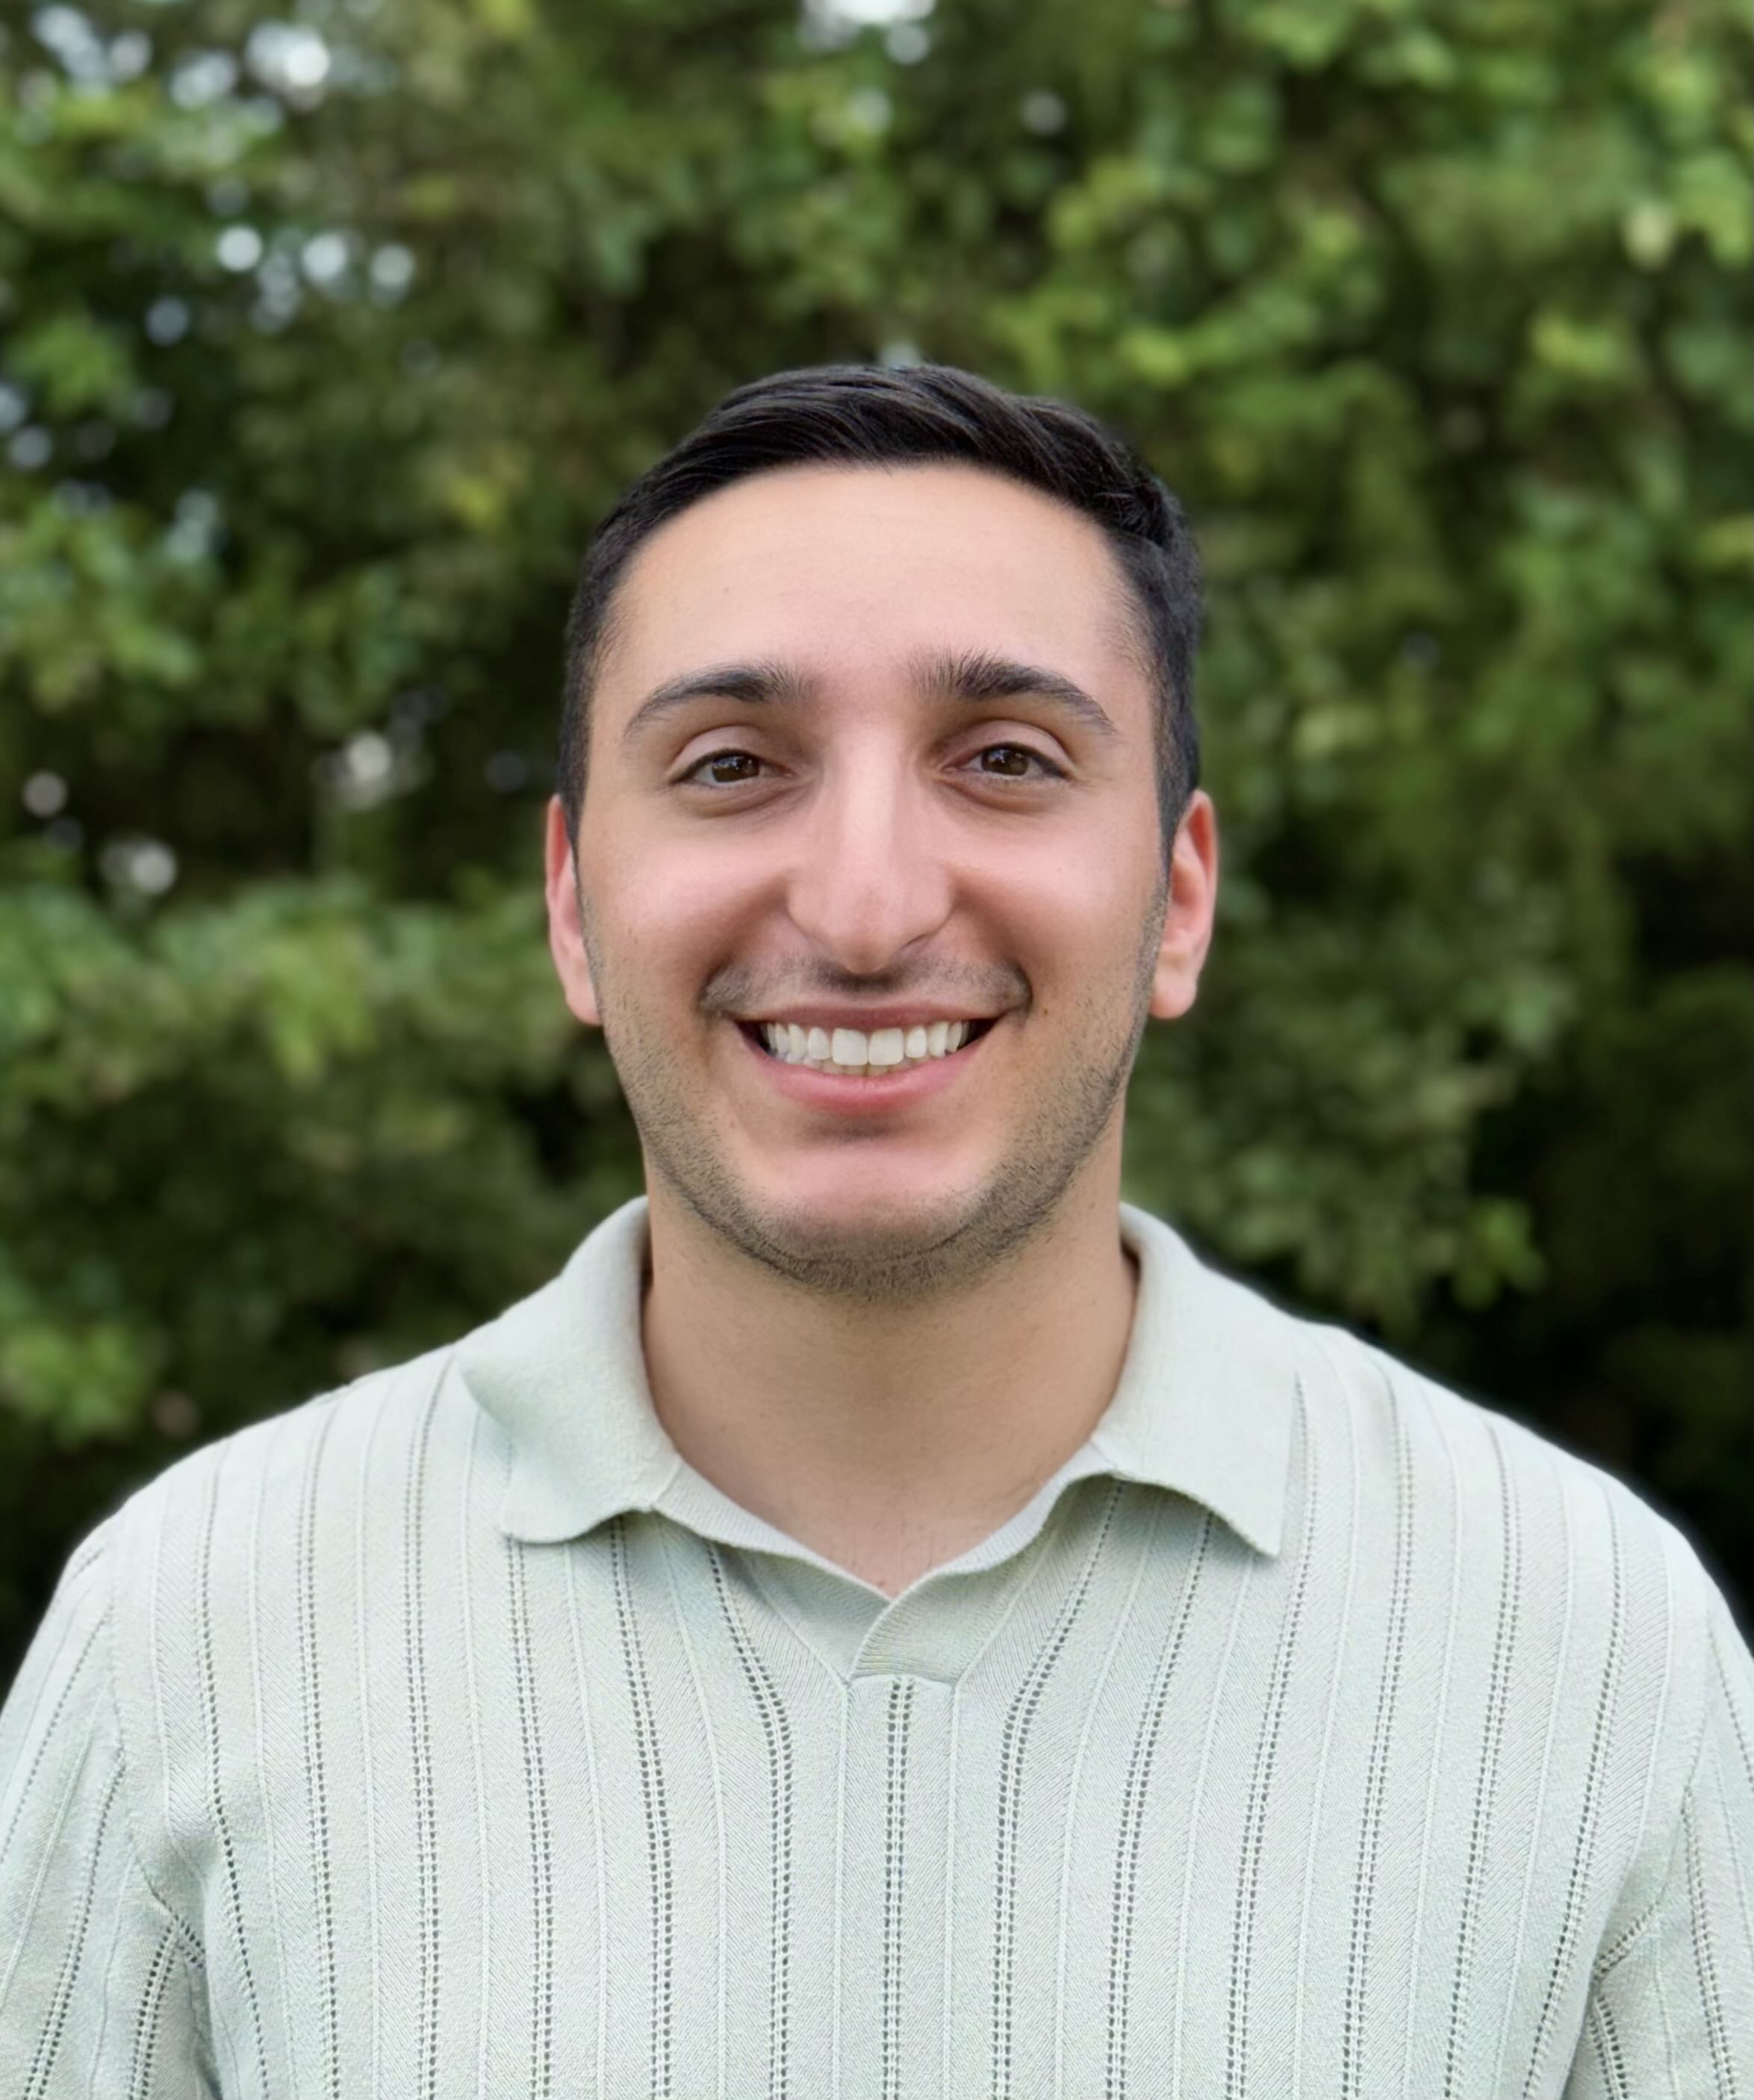
\includegraphics[width=\linewidth]{figures/headshot.png}
\caption[Example supplementary figure]{\textbf{Example supplementary figure.} This demonstrates how to include and reference supplementary material using a custom \texttt{supfigure} environment.}
\label{supfig:example_supp}
\end{supfigure}